\documentclass[10pt, conference, letterpaper]{IEEEtran}

\usepackage{times}		%% native times roman fonts
\usepackage{parskip}		%% blank lines between paragraphs, no indent
\usepackage[pdftex]{graphicx}	%% include graphics, preferrably pdf
\usepackage{amsmath}
\usepackage[pdftex]{hyperref}	%% many PDF options can be set here
\usepackage{amsthm,amssymb}
\usepackage{mathtools}
\usepackage[utf8]{inputenc}
\usepackage{stfloats}
\pdfadjustspacing=1		%% force LaTeX-like character spacing

\usepackage{listings}
\usepackage{color}

\definecolor{dkgreen}{rgb}{0,0.6,0}
\definecolor{gray}{rgb}{0.5,0.5,0.5}
\definecolor{mauve}{rgb}{0.58,0,0.82}

\lstset{frame=tb,
  language=Java,
  aboveskip=3mm,
  belowskip=3mm,
  showstringspaces=false,
  columns=flexible,
  basicstyle={\small\ttfamily},
  numbers=none,
  numberstyle=\tiny\color{gray},
  keywordstyle=\color{blue},
  commentstyle=\color{dkgreen},
  stringstyle=\color{mauve},
  breaklines=true,
  breakatwhitespace=true,
  tabsize=3
}

\hypersetup{
  pdfauthor = {Jos\'e Leal Domingues Neto},
}

\title{User-Level Location Aware Decision Engine for Mobile Computational Offloading}
\author{José Leal Domingues Neto \\ DCC, Universidade Federal de Minas Gerais \\ \href{mailto:joseleal@ufmg.br}{joseleal@ufmg.br}}

\begin{document}
\maketitle

\begin{abstract}
  Mobile computational offloading is a promising field in the area of mobile computing. Its benefits range from better responsiveness to less energy dependent applications. One of the big challenges in decent offloading frameworks is context-dependent dynamic evaluation of whether offloading at the moment is the right decision or not. This work proposes a user-level location aware decision engine for better bandwidth and execution time prediction. This proposed decision engine will not assume control over the mobile platform, being easily plugged into any offloading framework. This work develops a new black-box approach to estimate method execution time through little to no interference from the application developer. Additionally, it creates the possibility of choosing a ratio between responsiveness and energy saving. Experiments were conducted to test resource usage. Comparison showed that the version using this work used 50\% less battery.
\end{abstract}

\section{Introduction}

  Mobile devices cope with the difficult trade-off of providing high-end rich features and maintaining reasonable response time and battery life. Those devices follow the well known Moore's law, seeing processing and graphics power, storage capacity and high speed connectivity growing at fast pace while battery life does not tail such trend, becoming therefore a clear bottleneck \cite{Cuervo:2010:MMS:1814433.1814441}. Mobile computational offloading migrates pieces or possibly whole computational programs from the local processor to a less power limited platform e.g. a cloud computing environment \cite{Scavenger:5466972}. Offloading may reduce the response time and energy consumption on the mobile device.
 
 
  One of the most important tasks in offloading is the assessment of whether the device will profit by executing code locally or remotely. Although existing Cloud platforms are able to provision significant amounts of resources in very small time, the time to upload the code as to the Cloud and then to download the results may be longer than the time taken to perform the entire computation locally. Further, data transmission is a costly operation, specially in high data rate technologies such as 4G. As a consequence, computation and transmission times as well as energy consumption must be taken into account in offloading.
  
%  thus computation time as well as energy consumption must be taken into account. The energy consumption and processing delay dictate the success rate of offloading: If no energy and/or no time were saved in the operation, offloading does not make sense anymore. 
  
Most offloading frameworks employ as input parameters the available bandwidth and execution speed \cite{Cuervo:2010:MMS:1814433.1814441,Chun:2011:CEE:1966445.1966473,Shi:2014:CCO:2632951.2632958}, however they do not take into account that the bandwidth may change among cell towers and WiFi networks. This problem is exacerbated with Femtocells, since users are expected to roam among antennas more frequently.
 
Location should be taken into account when deciding to offload computation. Location directly affects properties such as energy consumption, round-trip time and available bandwidth. This means that the quality of experience (QoE) perceived by the user is also location dependent. When using the mobile device in an area with poor connectivity, the antenna has to be kept in a high energy state. The same applies for WiFi and mobile data. According to \cite{Schulman10bartendr:a}, six times more energy can be spent when transferring data in such situations. Existing frameworks do not account for location, resulting therefore in poor predictions in many cases.
   
 Exact geo-positioning, however, can be too costly or even unecessary. When the mobile device is connected to a cellphone tower, the tower identifier is available to the applications. This means that one can  correlate the tower identification with the user location. This information is more meaningful than the user's position, since the cellphone can be connected to several towers in a given location. In such cases, one tower can be completely overwhelmed while a nearby tower will provide an acceptable QoE. Thus,  knowing the exact geo-positioning of the user is usually not necessary. 
   
%   The LAC/CID of the tower, is therefore used as key to contextualize metrics. Clients connected to one tower will face similar connection speed.

This work improves the offloading decision by refining the assessment of the available bandwidth as well as energy consumption. This is achieved by two separate improvements. First, our method incorporates location awareness, identifying the cell tower or WiFi network and thus generating better estimations of the network condition. Second, we attempt to improve the modeling of the execution time of offloaded methods. Our framework treats the method as a black-box adjusting execution time as the input changes. In real world experiments, our approach proved to use 50\% less battery in the mobile devices for a face detection application.


%  This work also aims to solve one big issue with predictions: The runtime-execution of methods. Many of the projects use static profiling to assess code execution. The used metric is the number of instructions or simply the empirically measured execution time. This approach has many problems, as method execution is very dependent on inputs and the algorithm itself. 

The remainder of the paper is organized as follows. Section \ref{sec:related} discusses the related work. Section \ref{sec:design} presents the decision engine, detailing how it predicts the execution and transfer times, as well as how bandwidth is estimated. Section \ref{sec:setup} describes the experimental setup, and the results are discussed in Section \ref{sec:experiments}. Section \ref{sec:conclusion} presents the conclusions and future work.

\section{Related Work}
\label{sec:related}

  Much was invested in dynamic and static evaluation of offloading. Maui \cite{Cuervo:2010:MMS:1814433.1814441} offers a dynamic profiling mechanism called Maui Solver. It collects data for later assessment, taking RTT and bandwidth into account. These values are gathered and used as averaged estimates. We use a similar approach for these values when location cannot determined. CloneCloud \cite{Chun:2011:CEE:1966445.1966473} uses CPU activity, display state (on or off) and network state when deciding to offload. As said before, we will use network state and other inputs in our decision engine. ThinkAir \cite{kosta2012thinkair} has a comprehensive set of attributes monitored, checking battery level, data connectivity presence, connection type (WiFi, 3G, GPRS, UMTS), CPU activity, WiFi State (On/Off), perceived bandwidth, RTT and many others. We use a simpler model, reducing this set to avoid overhead. ThinkAir uses historical execution data for later predictions. Our decision engine uses more sophisticated algorithms to predict this, interpolating values as input varies.

  In the server-side, the COSMOS \cite{Shi:2014:CCO:2632951.2632958} project aims to manage the remote platform resources, diminishing costs by effectively allocating and scheduling offloading requests to reduce the monetary cost per request. This is an important issue, as we aim for a feasible solution, also in financial means. Other approaches aim the fast provisioning of servers to respond to the elastic demand of computational offloading frameworks \cite{Ha:2013:JPC:2462456.2464451}.

  Other works like \cite{6162380} exploit financial models, modeling therefore the offloading decision as a cost-effectiveness problem. 
  %This means that offloading will favor the most profitable choice at the moment, which in this case will be smartly modeled according to the problem. 
  This work has a similar framework, performing data fitting to obtain the utility functions and choosing the local optimal value in a greedy fashion. Scavenger \cite{5466972} creates a pervasive computing environment to make offloading possible. In this scenario, the client looks for services running in neaby devices and schedules tasks on those devices using RPC.

  For predicting future inputs ,\cite{Balan:2003:TRE:1066116.1066125,Cuervo:2010:MMS:1814433.1814441,kosta2012thinkair} draw a linear model of resource usage to extrapolate future values. This allows an approximate prediction of offloading inputs when they are not readily available or stale, such as bandwidth and method execution time. This paper improves those predictions by interpolating input values using a spline.

\begin{figure}[!t]
  \centering
  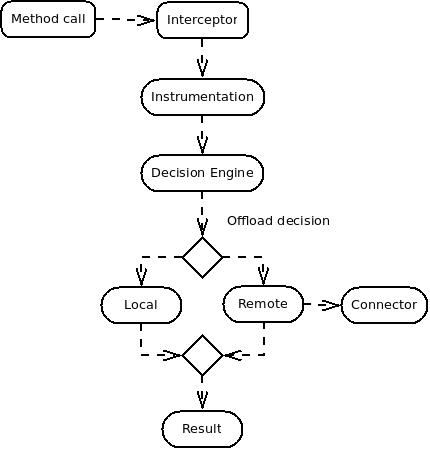
\includegraphics[width=0.35\textwidth]{imgs/diagram-complete.jpeg}
  \caption{Offload process}
  \label{fig:offloadprocess}
\end{figure}

\section{Proposed Offloading Decision} 
\label{sec:design}

  This project focuses on the offloading decision, however we describe the components of an offloading system before diving into the details of our solution. \ref{fig:offloadprocess} shows the components of an offloading framework. The {\it instrumentation component} will intercept and instrument the candidate methods for offloading. It receives annotated code, which marks the methods that are candidates for offloading. Whenever such methods are about to be executed, the instrumentation system calls the decision engine in order to determine if offloading should be performed. The instrumentation component also stores results of method execution times, network usage, partial calculations of bandwidth among others. The {\it decision engine} decides if offloading should be performed. In order to do so, it must estimate how much energy and CPU the method would consume if it were executed locally, as well as the time and energy required to transfer the method and its data to an offloading infrastructure.  The {\it connector module} is activated when offloading is performed, and takes care of remote connectivity and serialization/deserialization of objects.  The main contribution of this work is the decision engine, namely the use of location awareness in the offloading decision as well as the use of spline interpolation to better model the decision variables used by the engine.
  
  The proposed decision engine models the offloading problem using utility functions, and it is up to the user to decide if the engine should prioritize either reducing execution time or energy consumption. A constant, $\alpha, 0 \leq \alpha \leq 1$ is used for this purpose. A smaller $\alpha$ will make the decision tend towards saving energy. On the other hand, a bigger alpha will improve responsiveness. 

  The main equations for the boolean decision are presented below:
  \begin{equation} \label{eq:localutility}
    L(M) := \alpha \times tm_{l}(M) + (1-\alpha) \times en_{l}(M) 
  \end{equation}
  \begin{equation} \label{eq:remoteutility}
  \begin{multlined}
    R(M) := \alpha \times tm_{r}(M) + (1-\alpha) \times en_{r}(M) 
  \end{multlined}
  \end{equation}

  Where $M$ is the offloading candidate method, $L(M)$ is the estimated utility of local execution, and $R(M)$ is the utility of remote execution. The utility functions assess the time ($tm$) and energy ($en$) of the execution of $M$. Those functions will be detailed in section \ref{sec:time} and section \ref{sec:energy} respectively. To decide if the method should be offloaded, we compare the utility of local and remote executions as follows: 

  \begin{equation}
    decision(M) := R(M) < L(M)
  \end{equation}
  
  {\color{red} COMMENT: SINCE OFFLOADING CAN BE COSTLY/IMPRECISE, MAYBE WE COULD IMPROVE THIS EQUATION USING A HYSTERESIS VALUE, THAT IS:  R(M) + DELTA < L(M). THIS ENSURES THAT THERE IS A CERTAIN ADVANTAGE OF SENDING THE CALCULATION TO THE CLOUD.}

\subsection{Modeling Execution Time}
\label{sec:time}

 Execution time is hard to estimate. Mobile devices run several processes simultaneously. On top of that, the method to be offloaded is still a black-box and static profiling of code not always gives us useful hints. That means that better techniques ought to be developed.
  
  This paper introduces the concept of input assessment, in an attempt to model the execution time as a function of the arguments of a method. The concept is simple: A list of arguments of any type is converted to a unique numerical variable $assess(args)$. This variable will be directly proportional to the method's complexity. That means that given bigger assessments, the framework can expect that the method will take more time to finish. The decision engine analyzes annotations provided by the application developer, which are read in execution time. The annotations are used as a hint for the engine as to which variables are critical for the execution time of the method. Hard-coded types of variables are already available: if an \textit{integer} is annotated, its real value is summed to the assessment. If a \textit{string}, \textit{list} or \textit{set} is annotated, then its length is counted. If this behavior needs to be changed for a specific variable, or if non-standard types are used (such as custom classes), then the annotation can accept a class as an argument, which should implement an interface, converting this argument to a numerical value. The assessment is made at run-time. 

  The assessment value is then compared with the previous empirical execution times of the method. After five executions of the method, the decision engine starts to generate an interpolated curve of the execution time. The Akima Spline function was used as interpolator. Therefore, the local execution time $tm_{l}(M)$ is defined as follows:

  \begin{equation} \label{eq:timelocal}
    tm_{l}(M) := interpolate(M, Asm(M.args))
  \end{equation}
  \begin{equation}
    Asm(A) := \sum_{a \in A} assess(a)
  \end{equation}

The same approach is used for the remote execution time, gathering the execution time from the server and interpolating this value. On the remote platform we must take into account the additional uploading and downloading of the method's serialized arguments. To calculate this, location aware historical empirical data is used from past executions. Every time the method runs, location aware bandwidth is calculated and added to this database. The rule of thumb is: when on WiFi, bandwidth values from the same AP's \textit{MAC} address are used. When on mobile data, the tower's LAC/CID is recorded, together with its signal-to-noise ratio to later calculate expected bandwidth values.

It is not possible to interpolate values in the beginning, since the system does not have enough data. To circumvent this, the system initially checks if interpolation is possible at the time. If no, a random value $r$, $0 \leq r \leq 1$ is chosen. The response in these cases will be $decision(M) := r \leq 0.5$. That is, the system will randomly offload values in order to generate data until it can make a valid decision. This will of course depend of network state: If internet connectivity is not present, the decision will always be \textbf{not} to offload.

 To update the bandwidth values in the database, Equation \ref{eq:bandwidthup} is used to avoid drastic changes.

  \begin{equation} \label{eq:bandwidthup}
    b(t+1) = b(t) . (1-\beta) + value . (\beta), 0 \leq \beta \leq 1
  \end{equation}

  Finally the remote execution time follows equation \ref{eq:timeremote}.

  \begin{equation} \label{eq:timeremote}
    tm_{r}(M) := interpolate(M, Asm(M.args)) + trf(M.args)
  \end{equation}
  \begin{equation}
    trf(o) := size(o) / bandwidth
  \end{equation}

\subsection{Modeling Energy Consumption} 
\label{sec:energy}

  Many efforts were made to calculate energy from the mobile platform. The question still remains open, since there is still no precise way to calculate the method's energy consumption from a user-level point of view. The engine cannot gather this data precisely, therefore two assumptions are made: (a) Time is energy, so energy spent is directly proportional to time spent. (b) WiFi/Mobile Data energy usage can be modelled as a function of CPU energy usage. That means that using a modifier constant one can find a direct mapping between these values. This facilitates the normalization of the utility function, since it results on the same unit (time) when comparing CPU and time \cite{6606420}.

  The local energy consumption is therefore a sum of the CPU time spent, together with any data transferred by the method. This is  collected at runtime and interpolated following the approach presented for the execution time. In fact, two splines are created: one for execution time, the other for transferred data. This is done because of the black-box approach taken in this work. Equation \ref{eq:energylocal} presents the local execution time:

  \begin{equation} \label{eq:energylocal}
    en_{l}(M) := \\ tm_{l}(M) . C_{cpu} + dataTransferTime(M)
  \end{equation}

  Where $C_{cpu}$ is the modifier constant and $dataTransferTime(M)$ will deliver the interpolated value of the function's upload time. The remote counter-part of this equation contains similarly a constant $C_{radio}$ which normalizes the energy spent in radio transmissions, being the sum of transfer times of the method's serialized arguments and its result:

  \begin{equation} \label{eq:energyremote}
    en_{r}(M) := (trf(M.args) + trf(M.result)) . C_{radio}
  \end{equation}

  As mentioned above, the two modifier constants $C_{cpu}$ and $C_{radio}$ are used. They are necessary for a mapping between energy and time. Their values are empirical, and should be extracted from the data sheet of each device. One approach is to calculate those values and store them on a server, so the client application downloads the appropriate values based on the device's model and manufacturer. This avoids the intervention of the end-user of the device.

\subsection{Location Aware Bandwidth Prediction}

  When on cellular connectivity, the framework acts differently in order to predict real values for the current bandwidth. A slightly modified version of Shannon's equation is used, together with the current signal-to-noise ratio (SNR) acquired in real time from the mobile device, to estimate the user's bandwidth. This is required since a mobile tower server a much larger area than a WiFi access point, so the bandwidth varies significantly based on location. More formally, when receiving the perceived bandwidth $bw$, and the signal-to-noise ratio $SNR$, the LAC/CID from the current radio tower connected, a value $S$ is recorded in the database defined by:

  \begin{equation} \label{eq:shannonbw}
    S := bw * log_2(1 + SNR)
  \end{equation}

  The stored result will be then later retrieved to provide a location aware bandwidth, which will better describe the conditions at that location, taking into account the signal quality at the moment. To retrieve the bandwidth in a later time, the following reverse Shannon equation is used:

  \begin{equation} \label{eq:shannonbw_reverse}
    S' := S / log_2(1 + SNR)
  \end{equation}

  This way, a new educated guess is retrieved according to new values of $SNR$ and $S$ \ref{eq:shannonbw} at the tower. Upon receiving new data, this value is updated, thus maintaining the most actual state.
  
\subsection{Limitations of the Proposal}

As seen in this section, the proposed decision engine improves the state of the art by employing location awareness as well as refined methods to estimate the execution time of the methods. However, since the engine deals with estimations, it is important to discuss the limitations of the system.

The first aspect is the assessment of the execution time. The proposed assumes that larger inputs (e.g. larger integer numbers or larger vectors) will usually generate a longer execution time. This is a reasonable assumption for some problems. However, many problems do not follow such a premise, e.g. prime number calculation, where Mersenne  numbers (numbers in the form of $2^n-1)$ are much easier to check than ordinary numbers. 

Next, the offloading engine improves its decision with usage, since more data points will generate a more precise estimate. Thus, when more data points exists for the same method and the same location, the estimation will be improved. Conversely, calculations that are run occasionally will have worse predictions. One way to refine the decision is to use crowd sourcing, that is,  a server would aggregates the data points related to the execution of many users of one or more applications. This server would periodically upload to the mobile devices the most recent CPU execution curves and even the cellular speed estimates.

\section{Experimental Setup}
\label{sec:setup}

We created a full-sized Android application for recognizing faces to measure the effectiveness of the decision. The decision engine described in this work was used together with an Offloading Framework, which lies outside the scope of this paper, to test the predictions and correctness of the responses.

\subsection{Offloading framework}

We implemented an offloading framework for this paper. Our implementation does not require OS modifications on the mobile devices. As a consequence, it can be used directly in the user level, unlike some existing frameworks which require administrative privileges  \cite{Chun:2011:CEE:1966445.1966473}. Thus, an application developer could employ this framework to improve the responsiveness of its applications using cheap Cloud resources (e.g. using IaaS services so that the cost is a function of usage).

  The proposed offloading framework has a simple structure: (a) Post-compiler bytecode manipulator to inject method interceptors; (b) Remote execution platform running a Dalvik Virtual Machine \cite{ehringer2010dalvik}; (c) Offloading client library for server connection handling, serialization and deserialization, decision engine and instrumentation.  The decision engine described previously is plugged into (c). The remaining parts of the framework will be briefly explained for contextualization, but its scope differ from this project.

  The post-compiler bytecode manipulator receives an Android APK application as input and outputs a modified APK with the offloading stubs. It looks for the annotation "OffloadCandidate" in methods, creates a renamed copy of them, and modifies its body, adding the necessary calls for intercepting and triggering the decision engine. It then invokes the local or remote execution according to the output of the decision engine. The remote platform is composed of one or more servers running a DalvikVM. In each instance a server application receives pings and requests of clients. In case of requests for remote execution, it receives the serialized arguments, runs the given method and returns the output.

\subsection{Face Detection Application}
  
  An Android application for detecting faces on given images was created as a proof-of-concept. It receives an URL of an image, and then downloads it and detect the locations of faces on the object. Further on, it shows on the screen the faces delineated by a simple red square. A method that receives the image's internet address was created, outputting a byte stream with a downscaled image with the faces already marked by a red square. It was additionally annotated with the  "OffloadCandidate" annotation in order to be modified by the post-compiler.


\begin{figure}[!t]
  \centering
  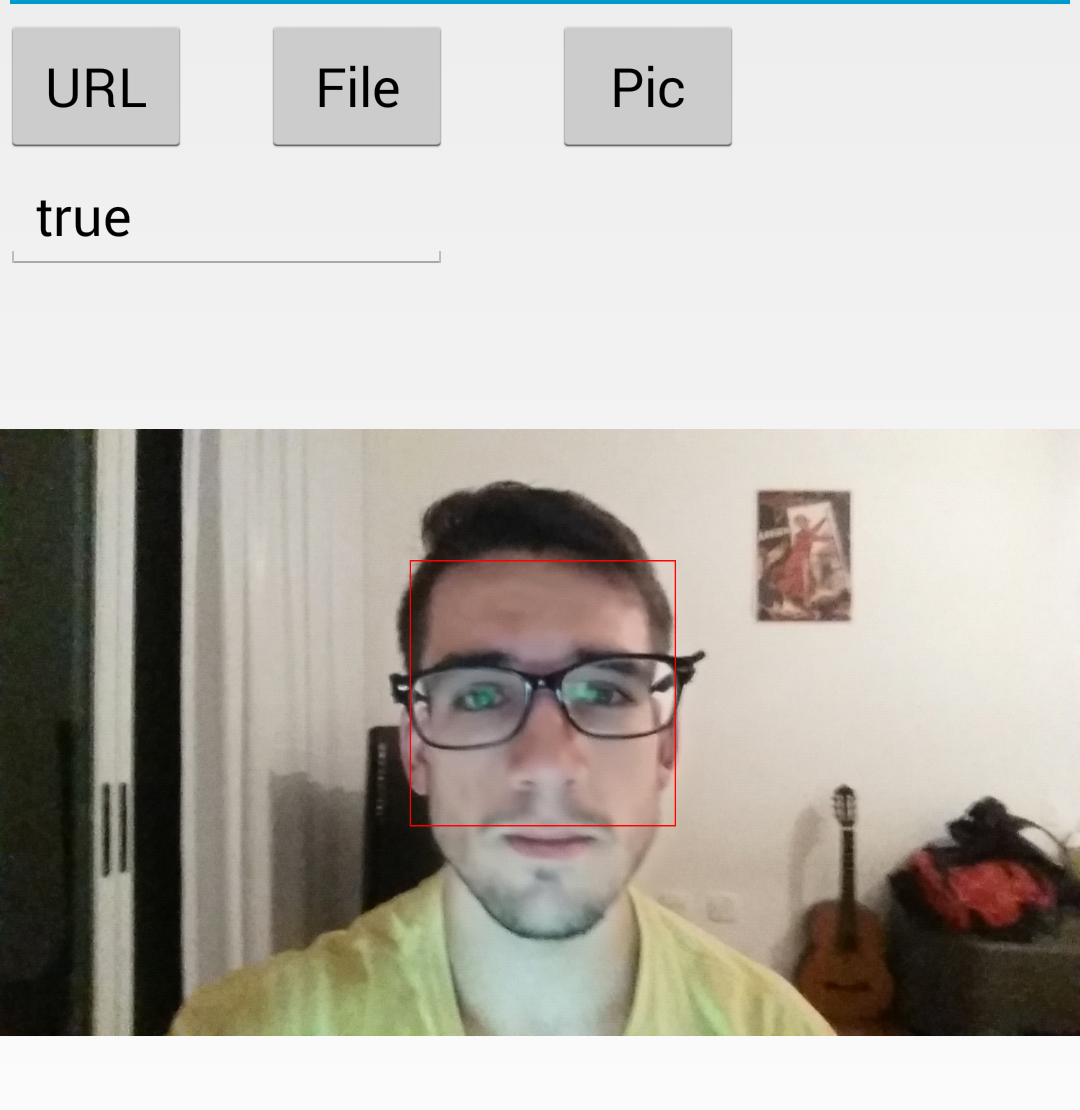
\includegraphics[width=0.4\textwidth]{imgs/app.png}
  \caption{Demo of the developed Android application.}
  \label{fig:exectime}
\end{figure}


  \subsection{Remote Platform}
  
  Several virtual machines instances can be created to serve requests according to demand, e.g. on a IaaS Cloud for usage-based billing. For this purpose, one instance was spun in DigitalOcean's infrastructure \cite{digitalocean} to be liable for requests. DigitalOcean offers IaaS (infrastructure as a service) virtual machines that are charged only for time used. We employed a VM having a 3GHz Intel Hexcore processor with 4GB of RAM. The server runs the DalvikVM with the server application (and Android emulator) in it, created using the Android AVD Manager \cite{androidavd} utility.

\subsection{Mobile platform}

  The mobile cellphone used for the tests was a Samsung Galaxy S5, which is powered by a Snapdragon 801 processor having a 2.5 GHz quad-core CPU and 2GB RAM. We can see that we are almost facing a technology convergence regarding computing power between the platforms. However, depending on context, the Snapdragon chipset can aggressively downscale the CPU speed and voltage to save battery, leading to energy savings at the cost of a reduced performance.

\section{Experiments}
\label{sec:experiments}
  
  The main goal is now to test whether the decision engine works under real life circumstances. The experiments were conducted in to order assess the differences between an application with and without the Offloading Framework. A version of the application including the framework and the decision engine of this project were used.

  A total of 36 image URLs were chosen, containing images from various sizes, colors and dimensions. Some of them contained a crowd with people whereas in others just one person. One can therefore test the performance of the methods and the correct instrumentation of each of them. The test consists of executing the method, providing these images in a cycle, 10 times in a row, occupying therefore the CPU and radio for about 20 minutes. The experiment evaluated the application using the decision engine, as well as the same application without offloading, under the same conditions. The tests were performed in a moving vehicle, communicating using an LTE Radio. The vehicle followed a pre-determined route, comprising of roads on the city center of Belo Horizonte, Brazil. Each run of the circuit was completed in roughly 20 minutes, and comprised 6.7km. Both versions of the application were run under normal battery conditions, with battery the saving mode disabled. The screen was maintained off the whole time and there were no other applications running on the background. The experiments were done using the values $\alpha = 1, C_{cpu} = 1, C_{radio} = 1$. The correct setting of these values will be better investigated in a future work.

\begin{figure}[t]
  \centering
  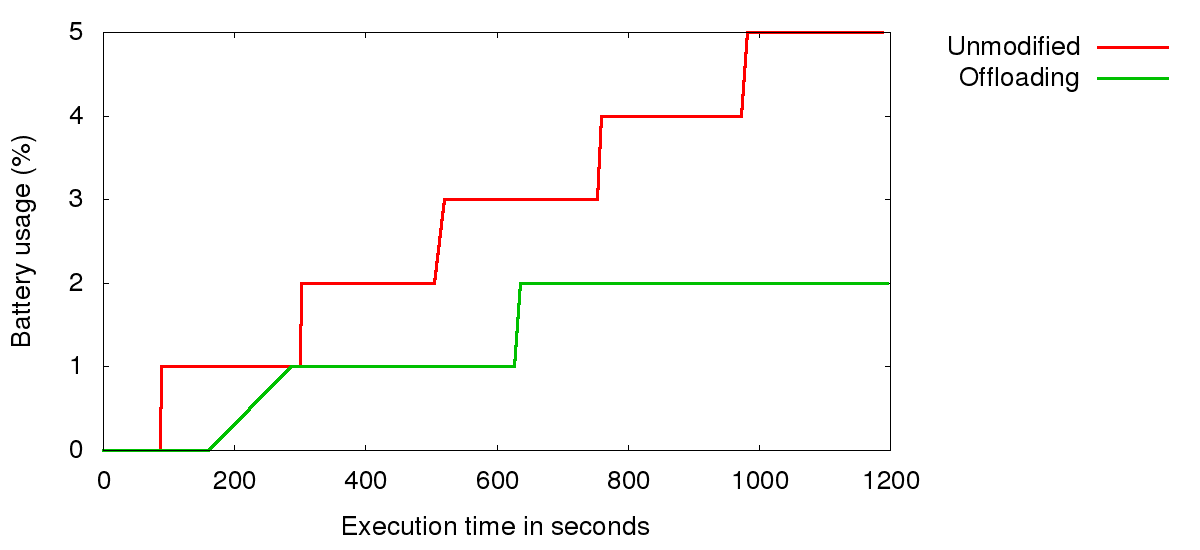
\includegraphics[width=0.5\textwidth]{results/plots/executions.png}
  \caption{Battery usage of the mobile device.}
  \label{fig:batteryusage}
\end{figure}

  \subsection{Energy Consumption Results}

The first test evaluated the energy consumption for a mix of large and small images, with a varied number of faces. The application, when using the Offloading Framework, used over 50\% less battery. Figure \ref{fig:batteryusage} plots the battery usage, showing that the offloading version presented a significantly softer energy discharge curve than the unmodified version. This can be explained by the data volume and CPU used by each one: cecause the Offloading version is not required to fetch the whole image directly, parse it and detect the faces on it, it will locally use less resources. Those results will be evaluated later on.

%The interesting scenario is when the image is relatively small and it is more efficient to simply download it directly and perform the work locally in the mobile. This may also happen when bandwidth is small.

\begin{figure}[t]
  \centering
  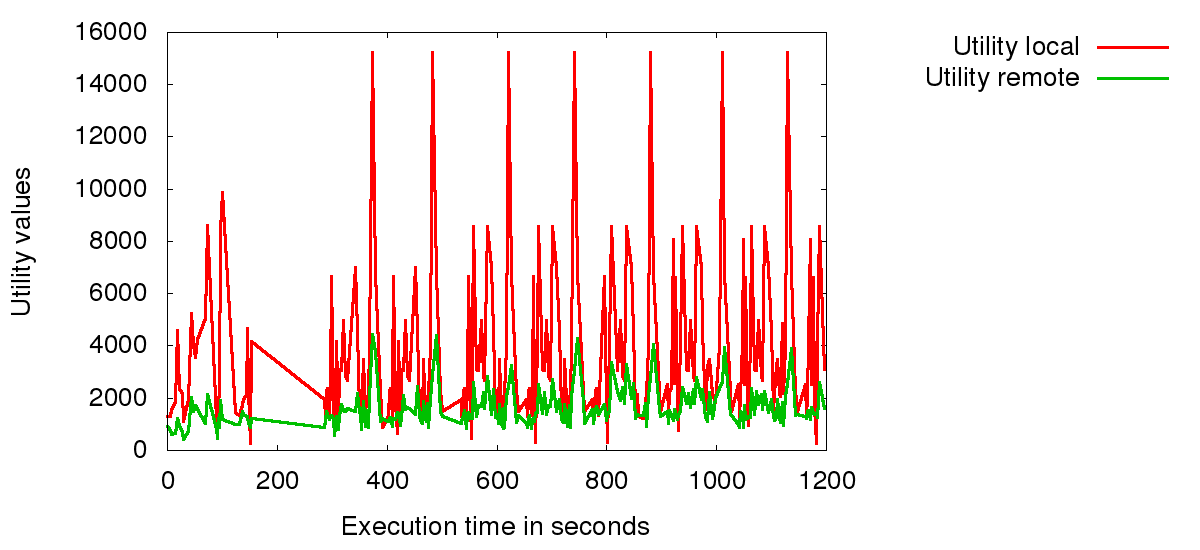
\includegraphics[width=0.5\textwidth]{results/plots/utility-fluctuation/executions.png}
  \caption{Values of the utility functions according to execution time. High and low peaks may mean different object sizes or bandwidth variation at the moment.}
  \label{fig:utilityplot}
\end{figure}

\subsection{Evaluating the Utility Functions}
  
This scenario analyzes the behavior of the utility curves.  As they are directly proportional to bandwidth, argument/result size and execution time, one can recognize the pattern of its curves. Figure \ref{fig:utilityplot} shows how the utility functions behaved during the tests. When the curve $L(M)$ is smaller than $R(M)$, the decision engine will execute the code locally. This happened a few times in specific images and situations. Looking at the oscillation of the curves, one can recognize different sizes of the objects. The high peaks mean big images, while the small ones are smaller ones, having conversely also a small utility value. Further,  the values of the local and remote utility curves arecomparable, having the curve of the remote utility function mirroring the local utility in smaller scale. 

  \begin{table}[t]
  \centering
  \caption{Example of evaluation of utility functions per image, \textbf{L} for local execution, \textbf{R} for remote}
  \label{table:utility}
  \begin{tabular}{rcrrcc}
    \textbf{Image size} & \textbf{Dimension} & \textbf{Local} & \textbf{Remote} & \textbf{BW (bps)} & \textbf{Decision} \\
   33kb & 416x300 & 287 & 880.30 & 12.74 & L \\
   28.9kb & 600x400  & 866 & 1237.59 & 7.80 & L \\
   545.8kb & 2000x1000  & 15231 & 3070.03 & 6.69 & R \\
   2.2mb & 1632x1226  & 32746 & 4288.64 & 12.03 & R \\
  \end{tabular}
  \end{table}

  Table \ref{table:utility} shows the evaluated utility equations per clusters of image, separated by their average image dimensions in pixels. Analyzing the patterns of the results, we can see that smaller images will be executed locally, as the local utility value is smaller than the remote one. If the image is fetched directly and locally processed it will consume less resources, thus offloading is not an efficient option. {\color{red} TODO: ANALIZE THE ACCURACY OF THE UTILITY CURVES. DO THEY PREDICT WELL THE FINAL VALUE OF THE EXECUTION AND ENERGY USAGE (WHAT WAS THE DEVIATION IN PERCENTS)? }

\subsection{Location Awareness}

One of the contributions of this paper is the location-aware modeling of the bandwidth. As explained before, the LAC/CID of the cell towers were stored together with its bandwidth in order to achieve faster convergence of bandwidth contextualized by location. Thus, in order to assess whether location was important, we measured the upload and download bandwidth of the LTE towers located during our experiments.  Figure \ref{fig:bwtime} shows the results. The assumption that bandwidth changes according to the cell tower proved to be correct, as its values varied for every tower. We can observe that the banwidth varied by as much as 61\% for download link, and 20\% for upload link. That is, we can see that the variation of upload link is much smaller. Further, Figure \ref{fig:bwtowers} presents the bandwidth variations over time. In  the figure, one can see these values according to cell tower and application execution time. Areas with different background color mean a tower change. 

\begin{figure}[b]
  \centering
  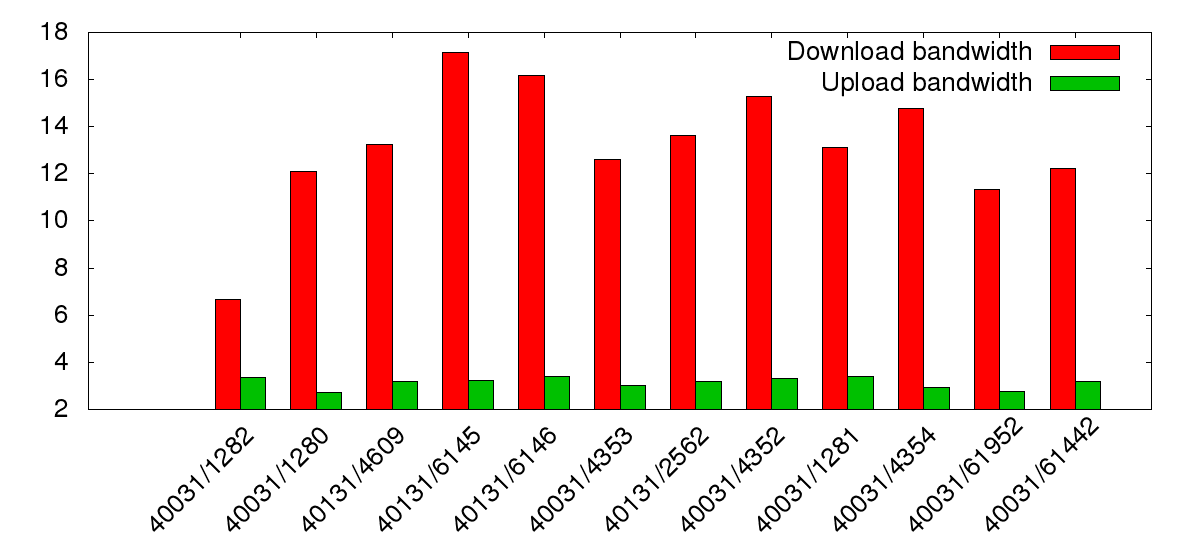
\includegraphics[width=0.5\textwidth]{results/plots/laccid-bw/bars.png}
  \caption{Bandwidth values for each LTE LAC/CID.}
  \label{fig:bwtime}
\end{figure}

\begin{figure}[b]
  \centering
  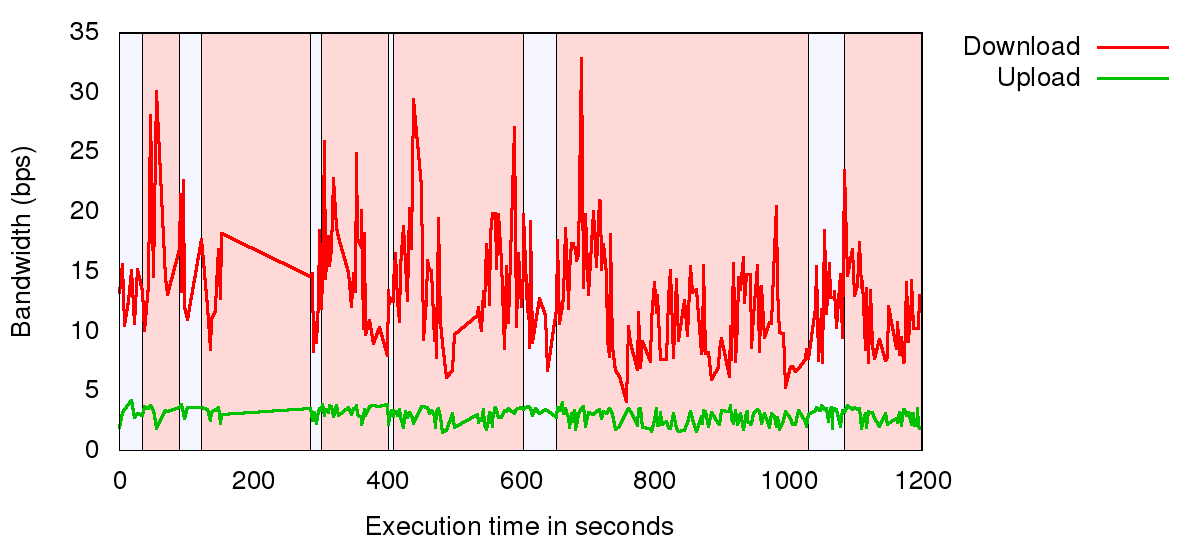
\includegraphics[width=0.5\textwidth]{results/plots/bw-fluctuation/executions.png}
  \caption{Bandwidth values over time during the experiment. Different background colors mean a cell tower change.}
  \label{fig:bwtowers}
\end{figure}

\subsection{System overhead}

To calculate the overall overhead of the proposed decision engine, two checkpoints were added outputting the delta of executions times, one right after the decision engine, and one right before the method result. The first checkpoint accounts to the total of $7.39\%$ in average of the whole process. The highest overhead was $21.89\%$. That means that most calculations are made with less than 10\% overhead. Figure \ref{fig:overheadexec} shows us the overhead values according to the total execution of each URL.

\begin{figure}[t]
  \centering
  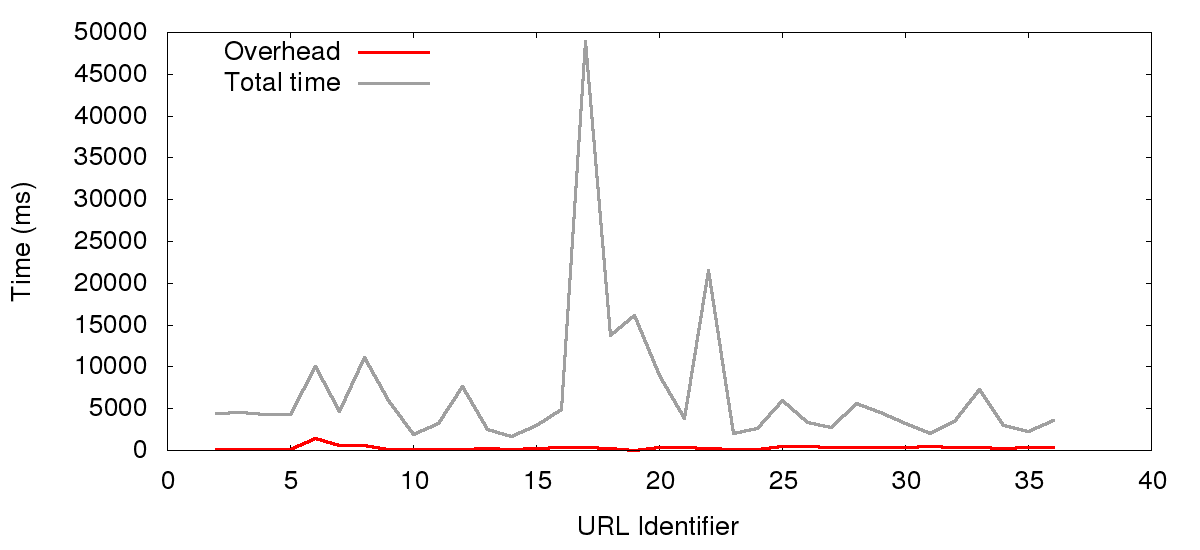
\includegraphics[width=0.5\textwidth]{results/plots/overhead/overhead.png}
  \caption{Overhead of the decision engine experienced in executions}
  \label{fig:overheadexec}
\end{figure}

 % Predicting the size of the result has also an impact in behaviour. It can be a turning point when compared to some method that may deliver a complex object. The remote platform could try to do a regression based on historical data and return the approximated result size in a later point, but currently it remains unknown until it is actually executed. For future executions, the assessment is used to retrieve this value in the future. I COMMENTED THIS PART BECAUSE IT IS A QUALITATIVE ASSESSMENT, WHICH DOES NOT PRESENT NUMBERS TO BACK THE CLAIMS.


  \subsection{Accuracy of the Utility Functions}

  In order to check the accuracy of the proposed model, the following steps were made:
  \begin{enumerate}
    \item With the results of the previous experiment already stored in the historical database, 4 unseen URLs were chosen.
    \item The Utility $L(M)$ and $R(M)$ were calculated for each of them.
    \item Additionally, the method was run on the local and remote platform separately and the execution times of each were computed.
  \end{enumerate}

Table \ref{table:correctness} presents the behavior of the utility function calculation.  As one can see, the overall error of the utility functions are relatively small. They succeed in modeling the problem correctly, pointing out when the local method will take less time. In some of the columns a bigger local utility value is perceived. That happens because the utility function consists of two parts, having as well energy being counted. In the remote counterpart, the values are significantly smaller for the energy function, as arguments and results set is the only element being counted there.


  \begin{table}[!t]
  \centering
  \caption{Correctness of utility functions, deviation of values between parenthesis}
  \label{table:correctness}
  \begin{tabular}{rcrrr}
    \textbf{ Img size } & \textbf{Local} & \textbf{Local Ut.} & \textbf{Remote} & \textbf{Remote ut.} \\
   100kb & 2600 & 1549 (40\%) & 2363 & 1350.18 (42\%) \\
   99.5kb & 2838  & 2539 (10\%) & 2549 & 1649 (35\%) \\
   104.7kb & 2734  & 2621.85 (4\%) & 1900 & 1222.88 (35\%) \\
   47.8kb & 1233  & 1307 (6\%) & 1320 & 1622.88 (22\%)
  \end{tabular}
  \end{table}

{\color{red}
Jose: We cannot really do this, because we don't have the necessary data for it. The 4 points available are the only (real measurements vs utility) we have so far.

HERE YOU CAN USE CLASSIC CURVE FITTING METRICS TO MEASURE THE EFFECTIVENESS OF THE UTILITY FUNCTION: 1 - R2. THE R2 COEFFICIENT MEASURES HOW MUCH OF THE DATA IS EXPLAINED BUY THE REGRESSION. HIGHER VALUES OF R2 MEAN THAT YOUR INTERPOLATION IS BETTER. 2 - RMS (https://en.wikipedia.org/wiki/Root\_mean\_square). THE ROOT MEAN SQUARE OF THE ERROR, THAT IS, THE ESTIMATED VALUE WHEN COMPARED TO THE ACTUAL VALUE. THIS IS ALSO A VERY IMPORTANT METRIC OF ACCURACY WHEN APPROXIMATING A FUNCTION.}

\section{Conclusions and Future Work}
\label{sec:conclusion}

Mobile computing devices are becoming pervasive, and application responsiveness as well as the mean time between battery charges are important metrics from the point of view of the consumer. One mean to improve both is the use of computation offloading, performing intensive computations on a Cloud infrastructure.

This paper presented a location-aware offloading framework for mobile devices. The framework improves the state of the art by taking location into account, as well as measuring the asymptotic runtime of methods using an assessment of the inputs. The proposed offloading framework does not need any special configurations nor modifications to the runtime of the remote platform, thus it can be easily plugged into any application. 

The framework was evaluated experimentally, using a face detection application. The results have shown that the battery usage can be greatly improved by efficiently offloading methods to a remote platform. Further, we also evaluated the effectiveness of the modeling, measuring the accuracy of the interpolations as well as whether the bandwidth actually changes among cell towers.

\subsection{Future work}
  The parametrization of the constants $C_{cpu}$ and $C_{radio}$ may not always model real world scenarios. For some cellphone chipsets, the energy spent function is not always linear, having sometimes the form of a ladder according to some situations, such as shutdown of cores or energy saving mode employed by them. Shannon's equation to predict bandwidth according to $SNR$ can also be improved in some cases. Although it depicts the bandwidth with very good approximation, it will output the upper bound of the connection capacity. Since LTE uses different modulations according to $SNR$, one good approach would be to retrieve these ranges and apply the capacity of theses modulations in respect to $SNR$. An eviction policy should be better applied in cases were the storage capacity of historical data is depleted. This can be a FIFO or a LRU data structure.

\bibliographystyle{unsrt}
\bibliography{parcial}

\end{document}
